\documentclass[a4paper,12pt]{article} 


\usepackage[T2A]{fontenc}			
\usepackage[utf8]{inputenc}			
\usepackage[english,russian]{babel}	

\usepackage{graphicx, scalerel}    
\usepackage{wrapfig}               
\usepackage[14pt]{extsizes}        
\usepackage[warn]{mathtext}       
\usepackage{indentfirst}      
\usepackage[margin = 25mm]{geometry}
\usepackage[table,xcdraw]{xcolor} 
\usepackage{amsmath,amsfonts,amssymb,amsthm,mathtools}
\usepackage{wasysym}                
\usepackage{upgreek}                
\usepackage{caption}
\usepackage{multirow}
\captionsetup{labelsep=period}
\usepackage[font=small,labelfont=bf]{caption}
\usepackage{gensymb}
\usepackage[unicode, pdftex]{hyperref}
\usepackage{tikz}
\usetikzlibrary{positioning}
\usepackage{fancyhdr}
\pagestyle{fancy}
\setlength\fboxsep{3pt} % Отступ рамки \fbox{} от рисунка
\setlength\fboxrule{1pt} % Толщина линий рамки \fbox{}
\setlength\extrarowheight{13pt}
\setcounter{secnumdepth}{0}

\begin{document}
		\newcommand{\HRule}{\rule{\linewidth}{0.7mm}} % Defines a new command for the horizontal lines, change thickness here

\begin{center}
	\large\textbf{Московский Физико-Технический Институт}\\
	\large\textbf{(государственный университет)}
	
	\vfill
	

	
	\Large Вычислительная математика
	%----------------------------------------------------------------------------------------
	%	TITLE SECTION
	%----------------------------------------------------------------------------------------
	
	\HRule
	\\[0.4cm]
	{ \huge \bfseries Лабораторная работа №9}
	\\[0.4cm] % Title of your document
	\HRule
	\\[0.5cm]
	
	\ \\
	\textbf{\large Автор:} \\	
	\large Овсянников Михаил Б01-008\\
	\vfill
	\hspace*{-0.8 cm}
\includegraphics[width=100 pt]{./Include/frkt_logo.pdf}\\
	\large Долгопрудный, 2023
\end{center}

\thispagestyle{empty}

\newpage
\setcounter{page}{2}
\fancyfoot[c]{\thepage}
\fancyhead[L] {Лабораторная работа №9}
\fancyhead[R]{}

		\tableofcontents
		\newpage
		
		\section*{Цель}
		\addcontentsline{toc}{section}{Цель}
		В работе предлагается вычислить производные некоторых функций численно и аналитически и сравнить результаты. Также, понять, какой метод имеет какой порядок точности, то есть $o(h^n)$, понять, какое $n$.
		
		
		\section*{Рабочие функции}
		\addcontentsline{toc}{section}{Рабочие функции}
		Нам дан список функций, для которых нужно провести данное исследование. Помимо этого также дан целый список методов аппроксимации производной функции в точке.  
		
		Перечислим все данные нам функции:
		\begin{itemize}
			\item $\sin(x^2)$
			\item $\cos(\sin(x))$
			\item $e^{\sin(\cos(x))}$
			\item $\ln(x + 3)$
			\item $(x + 3)^{0.5}$ 
		\end{itemize}
		
		Для дальнейшей работы нам понадобятся аналитические представления их производных, чтобы считать погрешность численного метода:
		\begin{table}[h!]
			\centering
			\begin{tabular}{|c|c|}
				\hline
				$f(x)$              & $f'(x)$                                         \\ \hline
				$\sin(x^2)$         & $2x\cos(x^2)$                                   \\ \hline
				$\cos(\sin(x))$     & $-\sin(\sin(x))\cos(x)$                         \\ \hline
				$e^{\sin(\cos(x))}$ & $e^{\sin(\cos(x))}\cos(\cos(x))\cdot(-\sin(x))$ \\ \hline
				$\ln(x + 3)$        & $\dfrac{1}{x+3}$                                \\ \hline
				$(x + 3)^{0.5}$     & $\dfrac{1}{2(x+3)^{0.5}}$                       \\ \hline
			\end{tabular}
			\caption{Таблица функция-производная}
		\end{table}
		
		Также нам даны различные методы численного определения производной. Перечислим и их тоже:
		\begin{enumerate}
			\item $f'(x) \simeq \frac{f(x + h) - f(x)}{h}$
			
			\item $f'(x) \simeq \frac{f(x) - f(x - h)}{h}$
			
			\item $f'(x) \simeq \frac{f(x + h) - f(x - h)}{2h}$
			
			\item $f'(x) \simeq \frac{4}{3} \cdot \frac{f(x + h) - f(x - h)}{2h} - \frac{1}{3} \cdot \frac{f(x + 2h) - f(x - 2h)}{4h}$
			
			\item $f'(x) \simeq \frac{3}{2} \cdot \frac{f(x + h) - f(x - h)}{2h} - \frac{3}{5} \cdot \frac{f(x + 2h) - f(x - 2h)}{4h} + \frac{1}{10} \frac{f(x + 3h) - f(x - 3h)}{6h}$
		\end{enumerate}
	
	
		Будем вычислять производную в какой-нибудь точке $x_0$ численно, затем аналитически и находить абсолютную погрешность численного метода $\varepsilon$.
		
		Также, будем менять шаг $h_n = \dfrac{2}{2^n}, \; n = \overline{1, 21}$ и смотреть, какова ошибка аппроксимации. Построим графики $\varepsilon(h_n)$ в логарифмическом масштабе по обеим осям - по наклону прямых поймем порядок точности метода.
		
		\newpage
		\section*{Графики и порядок точности}
		\addcontentsline{toc}{section}{Графики и порядок точности}
		Будем строить графики зависимости $\varepsilon(h_n)$ с помощью \href{https://www.python.org/}{Python}, а именно с помощью библиотеки \href{https://matplotlib.org/stable/tutorials/introductory/pyplot.html}{Matplotlib}. Весь код доступен в файле Lab1.py.
		
		Начальную точку выберем $x_0 = 10.0$. С помощью слайдера в программе можно менять точку, в которой считаются производные. С помощью кнопок можно переключаться между функциями, или же менять масштаб осей.
		
		\begin{figure}[h!]
			\centering
			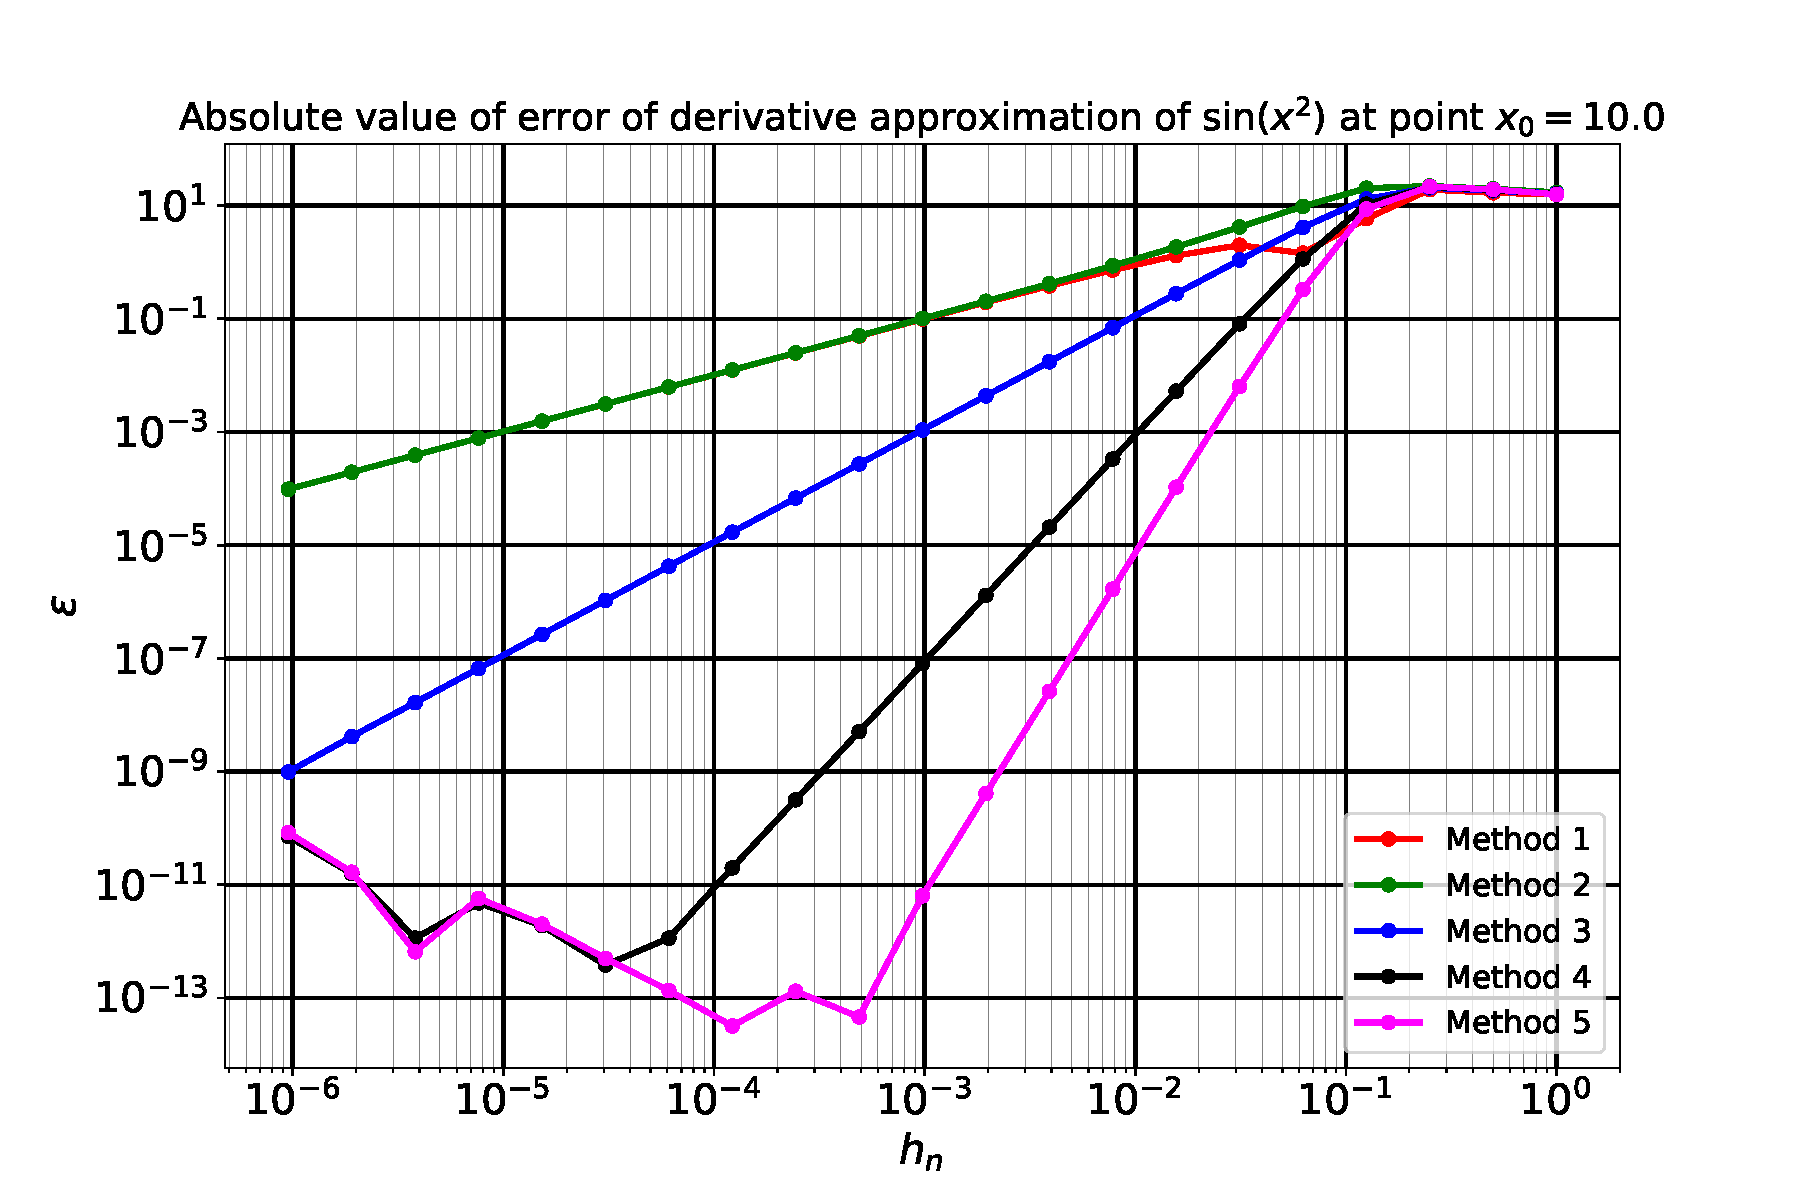
\includegraphics[width=\linewidth]{./Pictures/Function_1.pdf}
			\caption{Графики для функции $\sin(x^2)$}
		\end{figure}
	
		\newpage
		\begin{figure}[h!]
			\centering
			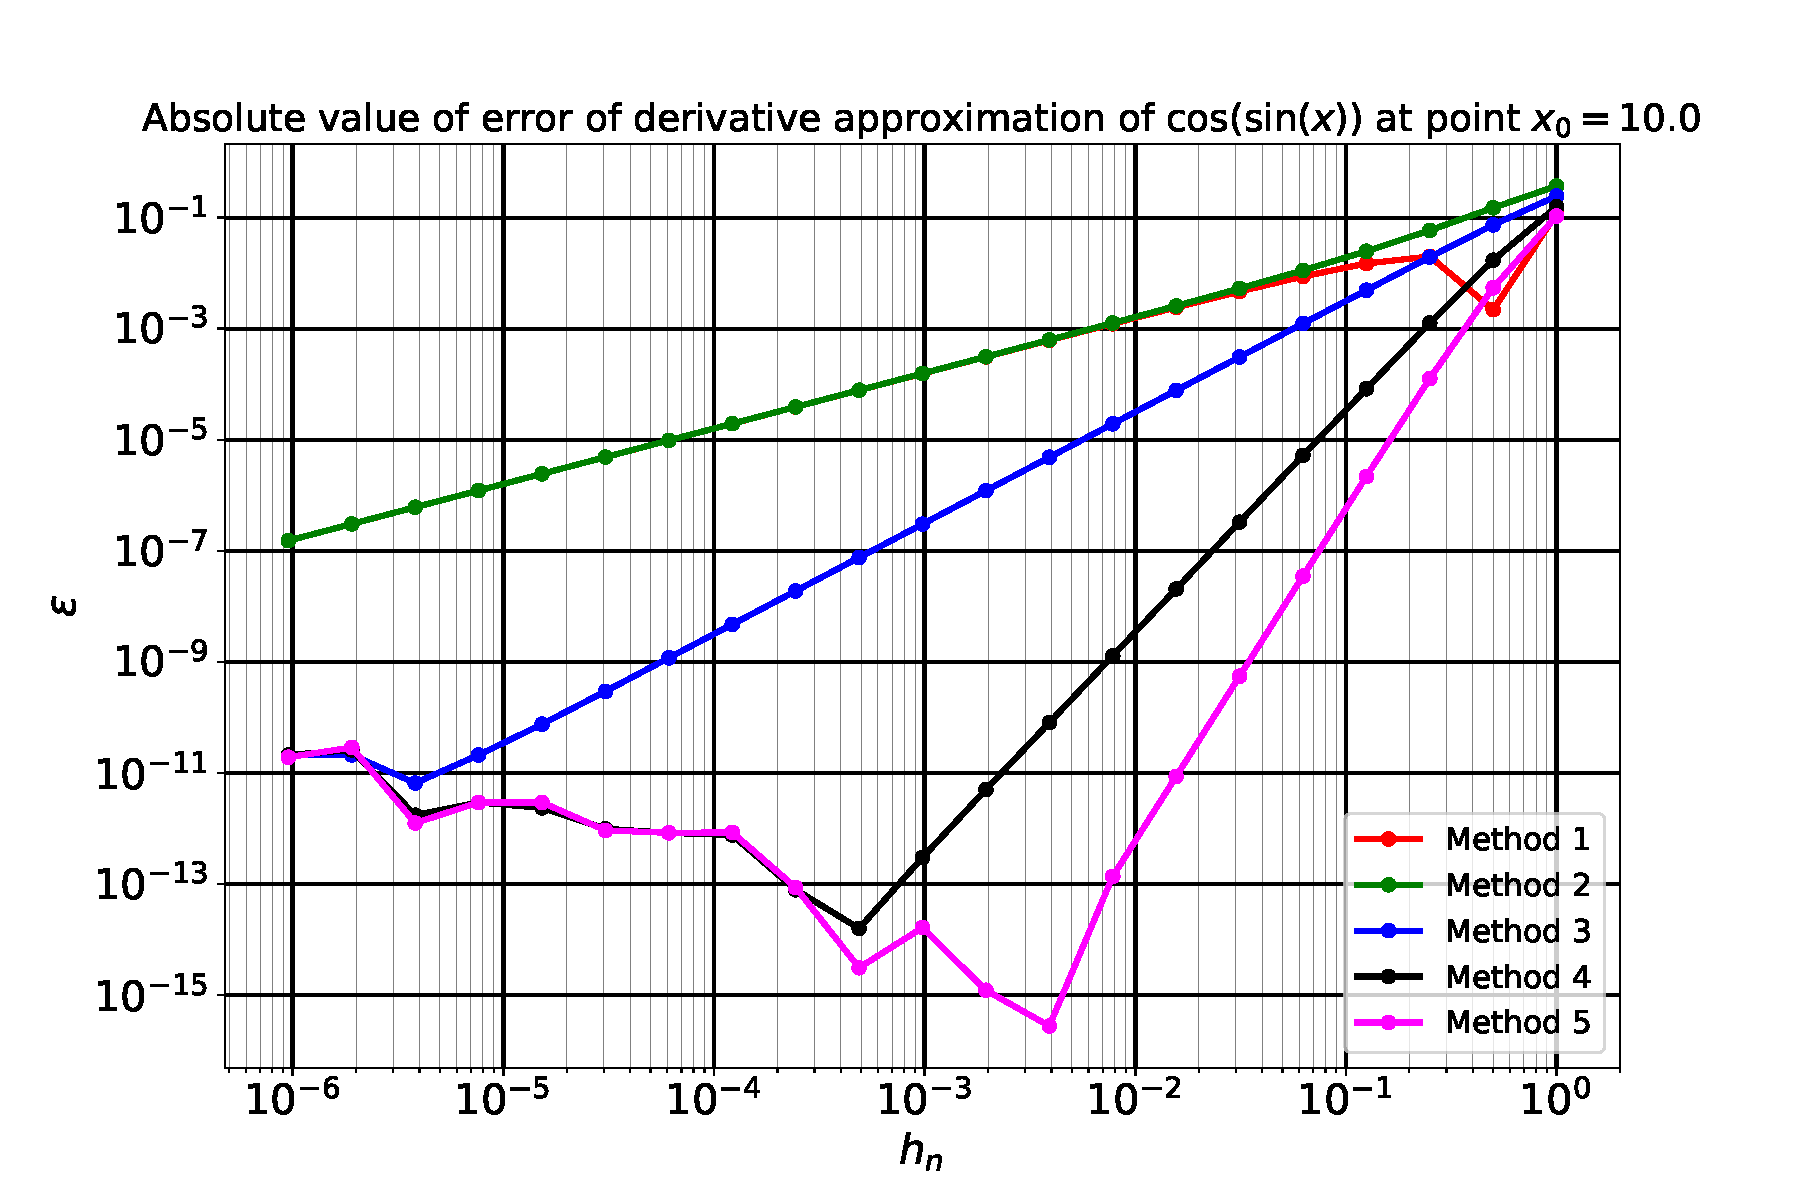
\includegraphics[width=\linewidth]{./Pictures/Function_2.pdf}
			\caption{Графики для функции $\cos(\sin(x))$}
		\end{figure}
	
		\begin{figure}[h!]
			\centering
			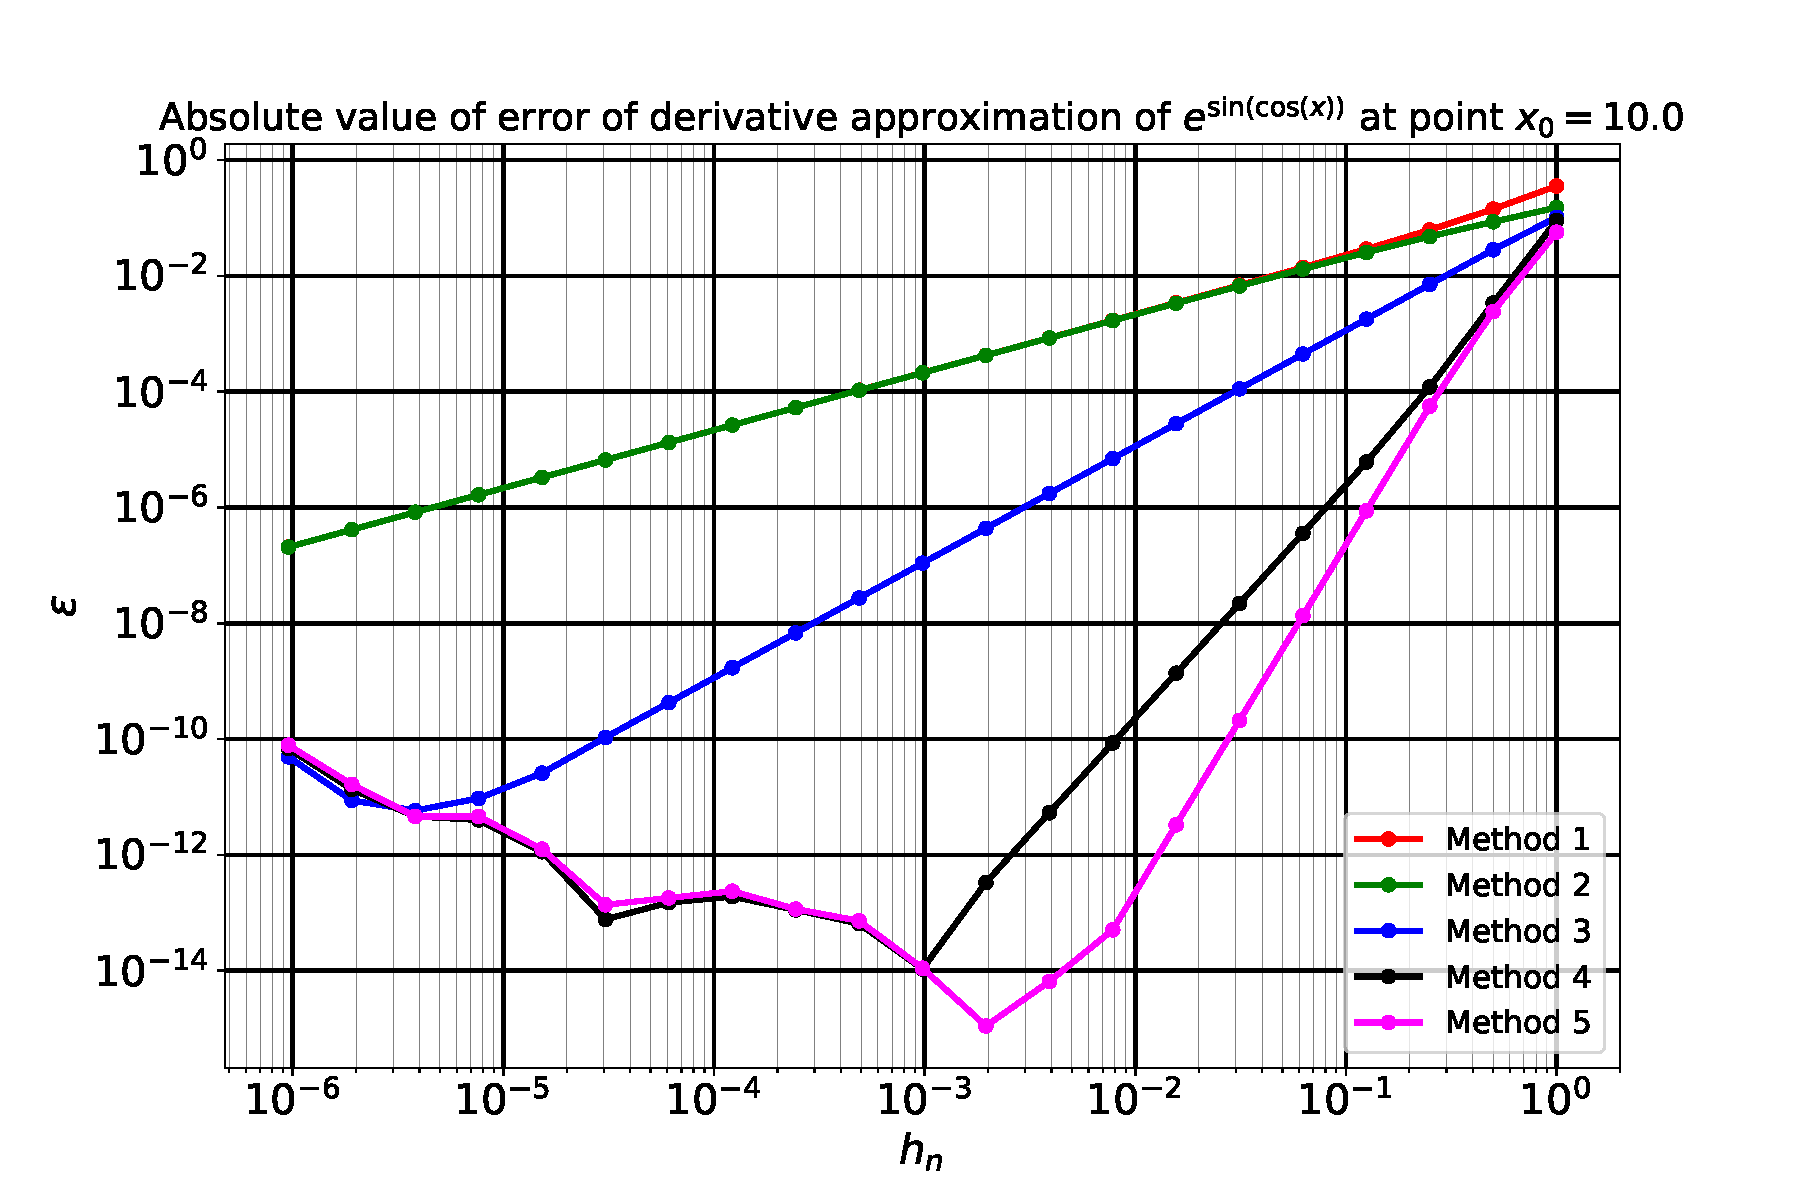
\includegraphics[width=\linewidth]{./Pictures/Function_3.pdf}
			\caption{Графики для функции $e^{\sin(\cos(x))}$}
		\end{figure}
	
		\newpage
		\begin{figure}[h!]
			\centering
			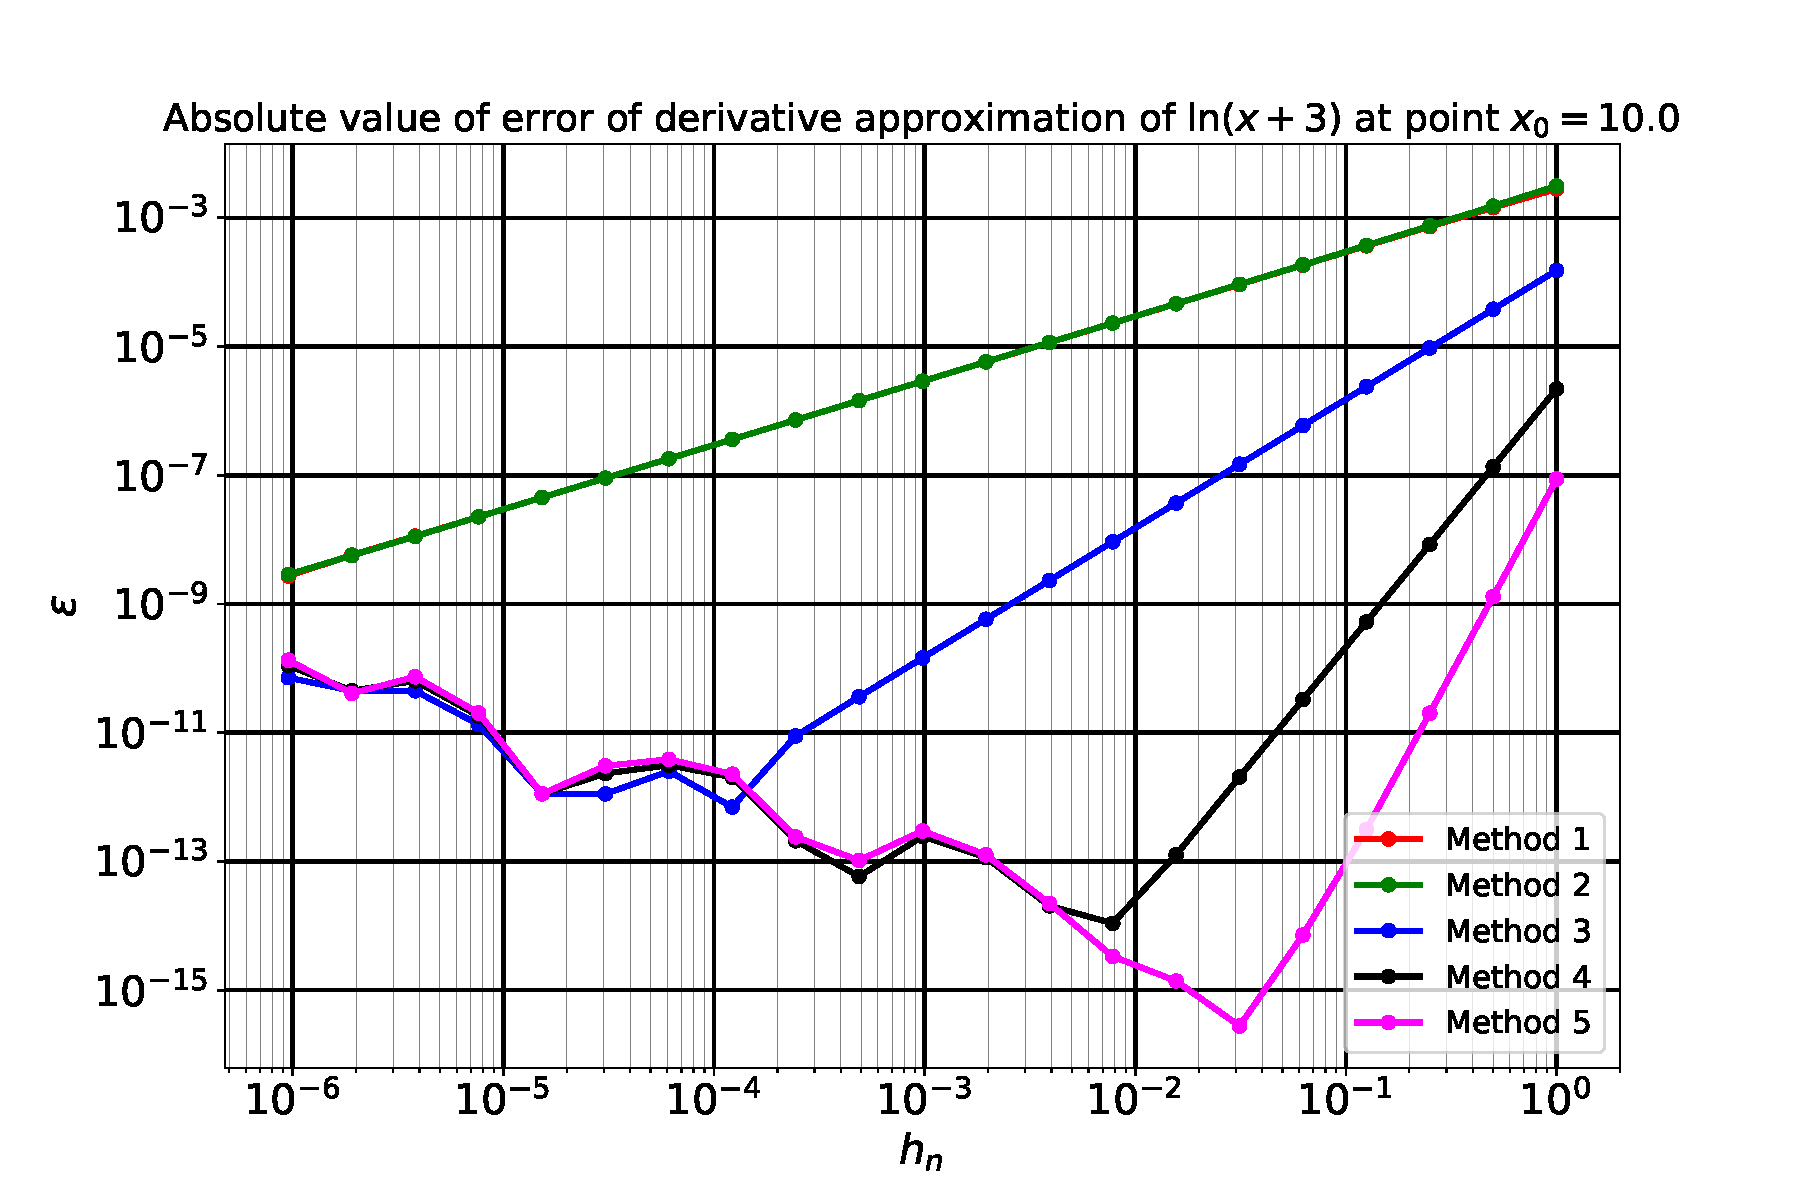
\includegraphics[width=\linewidth]{./Pictures/Function_4.pdf}
			\caption{Графики для функции $\ln(x + 3)$}
		\end{figure}
		
		\begin{figure}[h!]
			\centering
			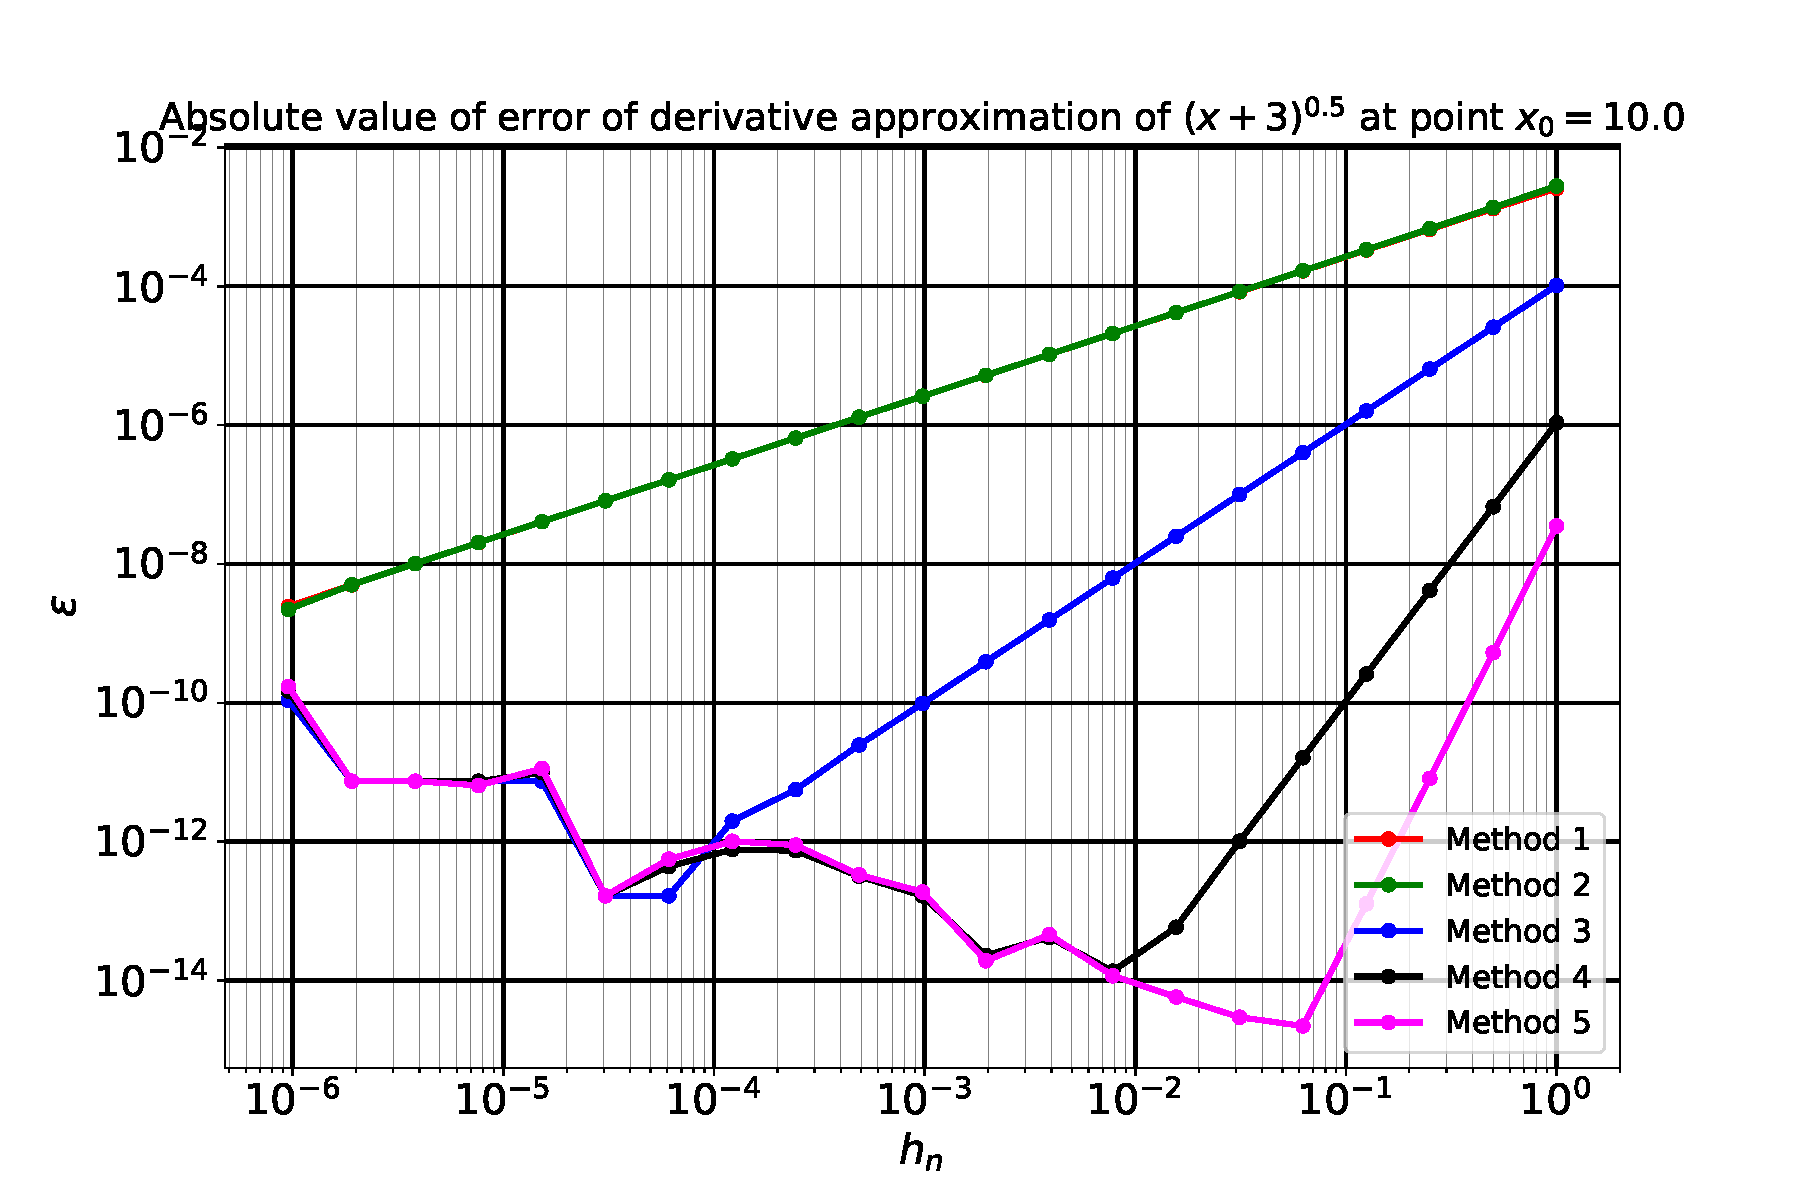
\includegraphics[width=\linewidth]{./Pictures/Function_5.pdf}
			\caption{Графики для функции $(x + 3)^{0.5}$}
		\end{figure}
 		
 		
 		\section*{Выводы}
 		\addcontentsline{toc}{section}{Выводы}
 		
 		По всем графикам видно, что общая точность растет с номером метода. По наклонам прямолинейных участков графиков можно заключить, что:
 		\begin{itemize}
 			\item Методы 1 и 2 имеют одинаковую точность $o(h)$
 			\item Метод 3 имеет точность $o(h^2)$
 			\item Метод 4 имеет точность $o(h^3)$
 			\item Метод 5 имеет точность $o(h^4)$
 		\end{itemize}
 	
 		Также на графиках отчетливо видно оптимальное значение шага $h$. Уменьшая шаг дальше, мы просто-напросто увеличиваем общую ошибку.
 		
\end{document}